Mes collègues développeurs étaient tous en alternance ou stagiaires.

J'ai du tout apprendre seul sur les documentations officielles des outils utilisés. En informatique, cela n'arrive jamais que l'on vous explique un outil. Les gens se forment tous seuls en allant lire.

Donc pour tout l'aspect purement fabrication du livrable nous étions seuls.

Cependant, la mission d'un ingénieur ne s'arrête pas simplement à l'execution de tâches. Pour tout ce qui vient en amont de la conception, c'est à dire le choix des technologies adaptées au besoin, comprendre le besoin exact, etc. Nous avons eu l'aide de \damien et \stefan.

Ils allaient en réunion avec le client et nous rapportait les besoins. \stefan s'est occupé de toute la partie UX du projet en decortiquant le besoin et en le transposant en maquette du livrable final. Cela nous a aidé à comprendre le vrai besoin métier derrière le projet bouclage de production.

En effet, ce que raconte le client dans son appel d'offre n'est pas forcément ce dont il a réellement besoin. Ici on partait tout de même d'une base d'un outil pré existant donc on pouvait également se servir de cela pour comprendre quels utilités ils en avaient chez SNCF.

\damien aussi permettait d'avoir une vision plus long terme du projet pour faire de meilleurs choix. Puisqu'il avait connaissance des 3 lots du projet avant même la signature de ceux-ci.

Pour résumé, j'ai effectué le travail de conception technique en totale autonomie (avec entraide avec les collègues évidemment). Par contre, sur toute la partie en amont de réflexion sur le projet, de comment articuler le besoin dans une application, quel choix de technologie faire, comment l'organiser. Là on a réfléchi avec \damien à cela. Et \stefan pouvait aussi nous donner son avis pendant l'avancement du projet grâce à son regard d'UX qui se doit de comprendre au moins le réel besoin métier derrière.

\begin{figure}[H]
    \centering
    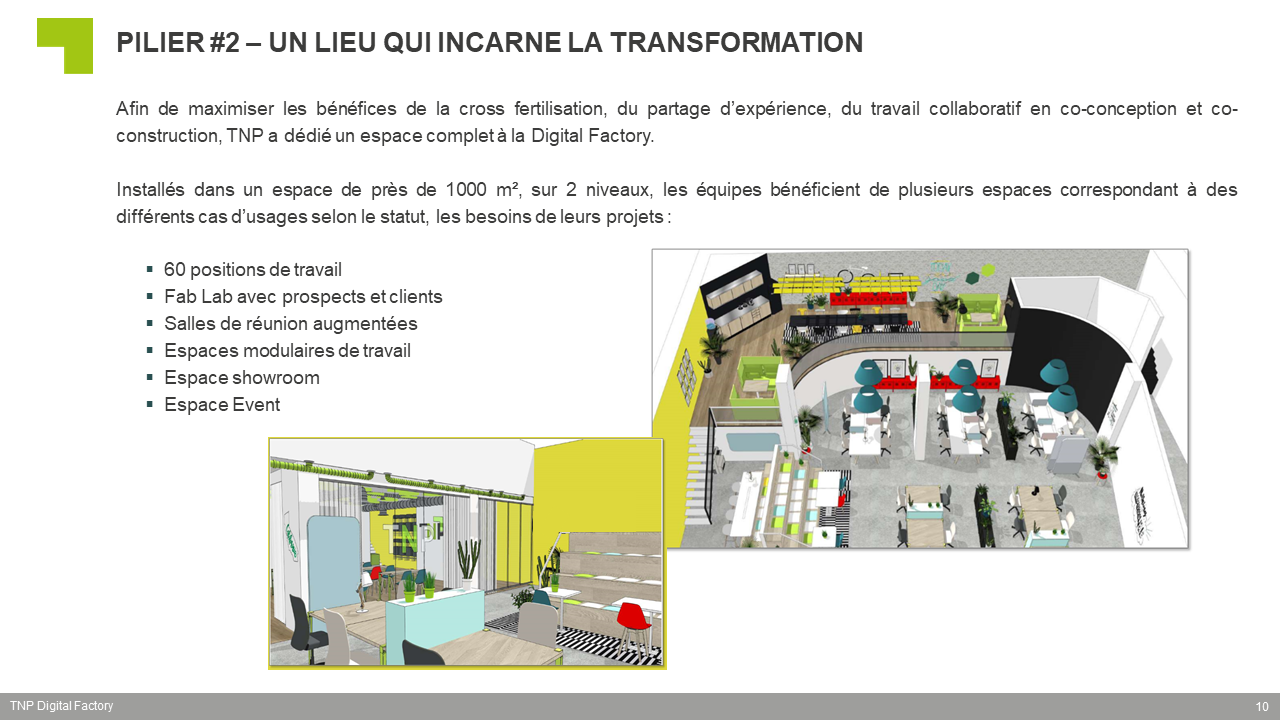
\includegraphics[width=.8\linewidth]{img/digital_factory_lieu.png}
    \caption{Présentation des bureaux de la Digital Factory}
\end{figure}

TODO parler des methodes de travail ? et de stefan ?
Et de l'equipe data science qui fait parti de la df

Et du gros boss de la df (sur les slides y'a son nom)